% Heizeinrichtung
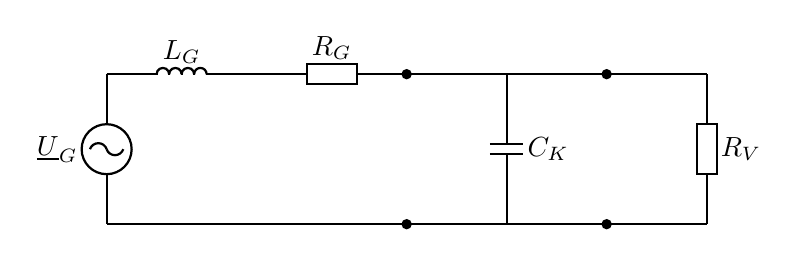
\begin{tikzpicture}[scale=2.54]%
% dpic version 2024.01.01 option -g for TikZ and PGF 1.01
\ifx\dpiclw\undefined\newdimen\dpiclw\fi
\global\def\dpicdraw{\draw[line width=\dpiclw]}
\global\def\dpicstop{;}
\dpiclw=0.8bp
\dpiclw=0.8bp
\dpicdraw (0,0)
 --(0,-0.25)\dpicstop
\dpicdraw (0,-0.375) circle (0.049213in)\dpicstop
\dpicdraw (-0,-0.375)
 ..controls (-0.005978,-0.357065) and (-0.022762,-0.344968)
 ..(-0.041667,-0.344968)
 ..controls (-0.060571,-0.344968) and (-0.077355,-0.357065)
 ..(-0.083333,-0.375)\dpicstop
\dpicdraw (0,-0.375)
 ..controls (0.005978,-0.392935) and (0.022762,-0.405032)
 ..(0.041667,-0.405032)
 ..controls (0.060571,-0.405032) and (0.077355,-0.392935)
 ..(0.083333,-0.375)\dpicstop
\dpicdraw (0,-0.5)
 --(0,-0.75)\dpicstop
\draw (-0.125,-0.375) node[left=-2bp]{$ \underline{U}_G$};
\dpicdraw (0,0)
 --(0.25,0)\dpicstop
\dpicdraw (0.25,0)
 --(0.25,-0.005556)\dpicstop
\dpicdraw (0.25,-0)
 ..controls (0.25,0.011165) and (0.255956,0.021481)
 ..(0.265625,0.027063)
 ..controls (0.275294,0.032646) and (0.287206,0.032646)
 ..(0.296875,0.027063)
 ..controls (0.306544,0.021481) and (0.3125,0.011165)
 ..(0.3125,0)\dpicstop
\dpicdraw (0.3125,0)
 --(0.3125,-0.005556)\dpicstop
\dpicdraw (0.3125,-0)
 ..controls (0.3125,0.011165) and (0.318456,0.021481)
 ..(0.328125,0.027063)
 ..controls (0.337794,0.032646) and (0.349706,0.032646)
 ..(0.359375,0.027063)
 ..controls (0.369044,0.021481) and (0.375,0.011165)
 ..(0.375,0)\dpicstop
\dpicdraw (0.375,0)
 --(0.375,-0.005556)\dpicstop
\dpicdraw (0.375,-0)
 ..controls (0.375,0.011165) and (0.380956,0.021481)
 ..(0.390625,0.027063)
 ..controls (0.400294,0.032646) and (0.412206,0.032646)
 ..(0.421875,0.027063)
 ..controls (0.431544,0.021481) and (0.4375,0.011165)
 ..(0.4375,0)\dpicstop
\dpicdraw (0.4375,0)
 --(0.4375,-0.005556)\dpicstop
\dpicdraw (0.4375,0)
 ..controls (0.4375,0.017259) and (0.451491,0.03125)
 ..(0.46875,0.03125)
 ..controls (0.486009,0.03125) and (0.5,0.017259)
 ..(0.5,0)\dpicstop
\dpicdraw (0.5,0)
 --(0.5,-0.005556)\dpicstop
\dpicdraw (0.5,0)
 --(0.75,0)\dpicstop
\draw (0.375,0.03125) node[above=-2bp]{$ L_G$};
\dpicdraw (0.75,0)
 --(1,0)\dpicstop
\dpicdraw (1.25,0)
 --(1.25,0.05)
 --(1,0.05)
 --(1,-0.05)
 --(1.25,-0.05)
 --(1.25,0)\dpicstop
\dpicdraw (1.25,0)
 --(1.5,0)\dpicstop
\draw (1.125,0.05) node[above=-2bp]{$ R_G$};
\dpicdraw[fill=black](1.5,0) circle (0.007874in)\dpicstop
\dpicdraw[fill=black](1.5,-0.75) circle (0.007874in)\dpicstop
\dpicdraw (1.5,0)
 --(2,0)\dpicstop
\dpicdraw (2,0)
 --(2,-0.35)\dpicstop
\dpicdraw (1.916667,-0.35)
 --(2.083333,-0.35)\dpicstop
\dpicdraw (1.916667,-0.4)
 --(2.083333,-0.4)\dpicstop
\dpicdraw (2,-0.4)
 --(2,-0.75)\dpicstop
\draw (2.083333,-0.375) node[right=-2bp]{$ C_K$};
\dpicdraw (2,0)
 --(2.5,0)\dpicstop
\dpicdraw[fill=black](2.5,0) circle (0.007874in)\dpicstop
\dpicdraw[fill=black](2.5,-0.75) circle (0.007874in)\dpicstop
\dpicdraw (2.5,0)
 --(3,0)\dpicstop
\dpicdraw (3,0)
 --(3,-0.25)\dpicstop
\dpicdraw (3,-0.5)
 --(3.05,-0.5)
 --(3.05,-0.25)
 --(2.95,-0.25)
 --(2.95,-0.5)
 --(3,-0.5)\dpicstop
\dpicdraw (3,-0.5)
 --(3,-0.75)\dpicstop
\draw (3.05,-0.375) node[right=-2bp]{$ R_V$};
\dpicdraw (3,-0.75)
 --(0,-0.75)\dpicstop
\end{tikzpicture}%
